%=================================================
\documentclass[12pt]{article}
\usepackage[left=3cm, right=2cm, top=3cm,bottom=2cm]{geometry}
\usepackage{fancyhdr}
\usepackage{listings}
\usepackage{float}
\usepackage[utf8]{inputenc}
\usepackage[brazil]{babel}
\usepackage{graphicx}
\usepackage{latexsym,amssymb,amsmath,amsfonts}
\usepackage{url}
\usepackage{indentfirst}
\usepackage{enumerate}
\usepackage{setspace}
\usepackage{placeins}
\usepackage{listings}
%\usepackage{minted}
 \usepackage{multirow}
\usepackage{subfigure}
\usepackage{enumitem}
\usepackage{subfigure}
\usepackage{wrapfig}
\usepackage{helvet}
\usepackage{epsfig}
%\usepackage{graphicx}
\usepackage{times}
\usepackage{arydshln}
\usepackage{subfigure}
\usepackage{amsmath,amssymb,amsthm}
\usepackage{graphicx}
\usepackage{lastpage}
\usepackage{multirow}
\usepackage{comment}
\usepackage[hidelinks]{hyperref}
\usepackage{placeins}
\usepackage{changepage}
%=================================================

\title{Processamento de Imagens}
\author{Paulo César Moraes de Menezes}
\date{\today}

\begin{document}

\maketitle

\newpage

\tableofcontents % Adiciona o sumário

\newpage

\section{Algumas informações iniciais sobre o documento}

Este documento terá todo o meu estudo direcionado ao tema de Processamento Digital de Imagens, a ideia é adicionar informações que foram
adquiridas tanto na disciplina Processamento de Imagens (DCE536) quanto em outras fontes de conhecimento.A ideia é que este documento seja
uma espécie de guia para o meu estudo, e que possa ser útil para outras pessoas que estejam interessadas no tema.
Além disso dedico o meu estudo para aprofundar o meu conhecimento em Inteligência Artificial, que é a área que pretendo seguir na minha
carreira profissional.

% Seu conteúdo aqui
\section{Créditos}

Algumas das informações presentes nesse documento foram extraídas do contéudo fornecido pelo professor Luiz Eduardo da Universidade Federal de
Alfenas.Quero agradecer a ele por compartilhar seu conhecimento na área.Além disso, algumas outras informações serão extraídas de fontes
externas, que serão devidamente referenciadas. Além disso, os textos são nota de base do livro "Digital Image Processing" de Rafael C. Gonzalez e Richard E. Woods.


\section{Introdução}



\subsection{O que é Processamento Digital de Imagens?}

Uma imagem pode ser definida como uma função de duas dimensões $f(x,y)$, onde $x$ e $y$ são coordenadas
espaciais em um plano e a amplitude de $f$ em qualquer par de coordenadas $(x,y)$ é chamada de intensidade
ou nível de cinza da imagem naquele ponto.Quando os valores de $x$, $y$ e $f$ são todos finitos e
discretos, chama-se a imagem de imagem digital.No que diz respeito ao campo de processamento digital
de imagens (PDI), o termo refere-se a processar uma imagem por meio de um computador digital.É válido
destacar que uma imagem digital é composta por finitos elementos, cada elemento possuí um valor de
intensidade e posição associado a ele.

Com essas informações em mente, também é válido destacar um dos grandes responsaveis por dar vida a
capacidade de reconhecer imagens: a visão humana.A visão humana é um dos grandes sentidos que o ser
humano possuí, e é também um dos mais complexos.A visão é capaz de capturar e processar
informações visuais de forma extremamente rápida e eficiente.Entretanto, a visão humana não é perfeita, e
também possuí limitações, como por exemplo não ser capaz de enxergar certos comprimentos de onda de
luz, ou ser limitado pelo espectro EM (Eletromagnético) que é capaz de capturar.

Contudo, as máquinas conseguem capturar quase todo o espectro EM, e com isso é possível processar
imagens de forma extremamente eficiente, e é aí que entra o Processamento Digital de Imagens, que é a
área que estuda técnicas e métodos para processar imagens de forma eficiente, e é uma das áreas que
possuí grande importância na área de Inteligência Artificial, pois é uma das áreas que estuda a
capacidade de reconhecer padrões em imagens, que é uma das capacidades que o ser humano possuí.

As máquinas conseguem operar em faixas de frequência que o ser humano não consegue, como por exemplo
raios-x, raios gama, entre outros.

É comum existir um debate do que seria processamento de imagens e visão computacional.Esse debate é
comum, pois as duas áreas possuem muitos pontos em comum, e muitas vezes são utilizadas de forma
intercambiável, entretanto, é válido destacar que as duas áreas possuem diferenças, e que a visão
computacional é uma área que estuda como as máquinas podem ser capazes de interpretar e entender o
mundo visual, enquanto que o processamento de imagens é uma área que estuda como as imagens podem ser
processadas de forma eficiente.O processamento de imagens concentra-se principalmente em técnicas e algoritmos para manipular e
melhorar imagens digitais.Isso inclui operações como filtragem, realce de borda, remoção de ruído,
entre outros, com o objetivo de melhorar a qualidade ou extrair informações úteis das imagens.


 \subsubsection[Processos de baixo nível]{Processos de baixo nível}
Esses processos são conhecidos também como processos primitivos ou pré-processamento, e são processos
para reduzir ruído, realçar bordas, corrigir desfoque, entre outros.

Um processo de baíxo nível é caracterizado pelo fato de que a sua entrada e saída são imagens, e que
não existe um conhecimento prévio sobre o conteúdo da imagem, ou seja, o processamento é feito de forma
cega, sem saber o que está sendo processado.

 \subsubsection[Processos de médio nível]{Processos de médio nível}

O processo de médio nível envolve técnicas de segmentação, que é o processo de dividir a imagem em
partes, ou seja, é o processo de dividir a imagem em partes que são de interesse, e partes que não são
de interesse.Essa segmentação pode ser feita separando a imagem em regiões ou em objetos.Além disso
esse tipo de processo envolve uma descrição sobre os objetos segmentados de modo a reduzi-los de uma
forma adequada para o processamento computacional e a classificação de objetos individuais.

Além disso uma outra característica desse tipo de processo está no fato de que as entradas são
imagens, mas as saídas são atributos extraídos dessas imagens, como por exemplo, a forma, a cor, a
textura, entre outros.

 \subsubsection[Processos de alto nível]{Processos de alto nível}

Esse tipo de processo envolve dar sentido ao conteúdo da imagem, ou seja, envolve a interpretação do
conteúdo da imagem, e é um dos processos mais complexos, e que envolve a utilização de técnicas de
inteligência artificial, como por exemplo, redes neurais, entre outros.

\subsection{As origens do Processamento Digital de Imagens}

Uma das primeiras aparições das imagens digitais foi no jornal industrial no começo dos anos 1920,
na qual foi enviado através de submarinos entre Londres e Nova York, e foi a primeira vez que uma
imagem foi transmitida de forma eletrônica.Esse feito reduziu para horas um trabalho que levava
semanas para ser feito.

\begin{figure}[h]
  \centering
  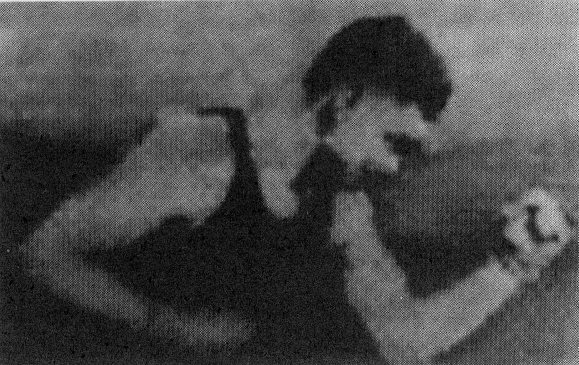
\includegraphics{images/3 2}
  \caption{Imagem digital produzida por fita codificada.}
  \label{fig:exemplo}
\end{figure}

Essas capturas pioneiras tinham capacidade de reconhcer até 5 tons de cinza.Esse valor foi aumentando
até que em 1929 alcançou a incrível marca de 15 tons de cinza.

Um grande fator que limitou o avanço das imagens digitais foi a falta de tecnologia para armazenar
essas imagens, é nítida a relação de dependência entre poder computacional e armazenamento de imagens.

Ao longo do século XX, o PDI foi se desenvolvendo, e foi se tornando uma área de grande importância
para a sociedade, e com a medida que a técnologia computacional evoluia, principalmente durante a
corrida espacial, o PDI foi se tornando uma área de grande importância para a sociedade.


\begin{figure}[h]
  \centering
  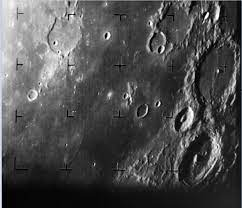
\includegraphics{images/2}
  \caption{Primeira imagem digital da Lua, em 1964.}
  \label{fig:exemplo}
\end{figure}

Além disso, durante a década de 70, o PDI começou a ter aplicações em medicina, e com isso o PDI
começou a ter um grande impacto na sociedade, principalmente com o desenvolvimento de Tomografias
Computadorizadas, que é uma das grandes aplicações do PDI.

\subsection{Aplicações do Processamento Digital de Imagens}

Atualmente praticamente todas as áreas da sociedade possuem aplicações do PDI, e é uma área que
exerce grande influência na sociedade.

\subsubsection{Imagens Raio-Gamma}

A vasta maioria dos usos nesta área é para aplicações de medicina nuclear e observações astronômicas.

A ideia para a medicina nuclear é aplicar isótopos radioativos em um paciente, e com isso é possível
observar o decaimento desses isótopos.Desse modo, é possível coletar imagens do interior do corpo
humano, e com isso é possível diagnosticar doenças.

\begin{figure}[h]
    \centering
    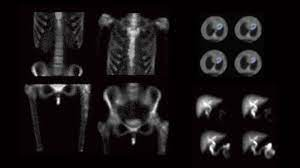
\includegraphics{images/3.jpeg}
    \caption{Gamma Ray Image}
    \label{fig:exemplo}
\end{figure}

\subsubsection{Imagem de Raio-X}

Esta é uma da aplicação mais antigas do PDI, e é uma das aplicações mais conhecidas do PDI.Usada princi
palmente para diagnóstico médico, mas pode ser utilizada em outras áreas, como por exemplo, para
inspeção de bagagens em aeroportos.

\begin{figure}[h]
    \centering
    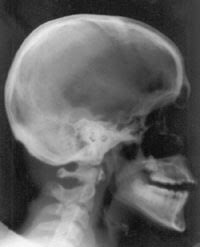
\includegraphics{images/4.jpeg}
    \caption{Raio-X}
    \label{fig:exemplo}
\end{figure}

\section{Fundamentos de Imagens Digitais}

\subsection{Elementos da percepção visual}

É notório que, baseado no que foi visto até então, o campo do processamento digital de imagens é baseado
em alguns elementos matemáticos e fisícos, entretanto a análise e a intuição humana de como as coisas
funcionam é de grande importância para o desenvolvimento de algoritmos e técnicas de processamento de
imagens.

Com isso em mente é fundamental compreender as limitações da percepção humana, e como a percepção
humana é capaz de interpretar e entender o mundo visual.

\subsubsection{A visão humana}

A figura 5 exemplifica a seção transversal do olho humano.O olho é quase uma esfera, com diâmetro
aproximado de 24mm.

Três membranas principais cobrem o olho:


\begin{figure}[h]
    \centering
    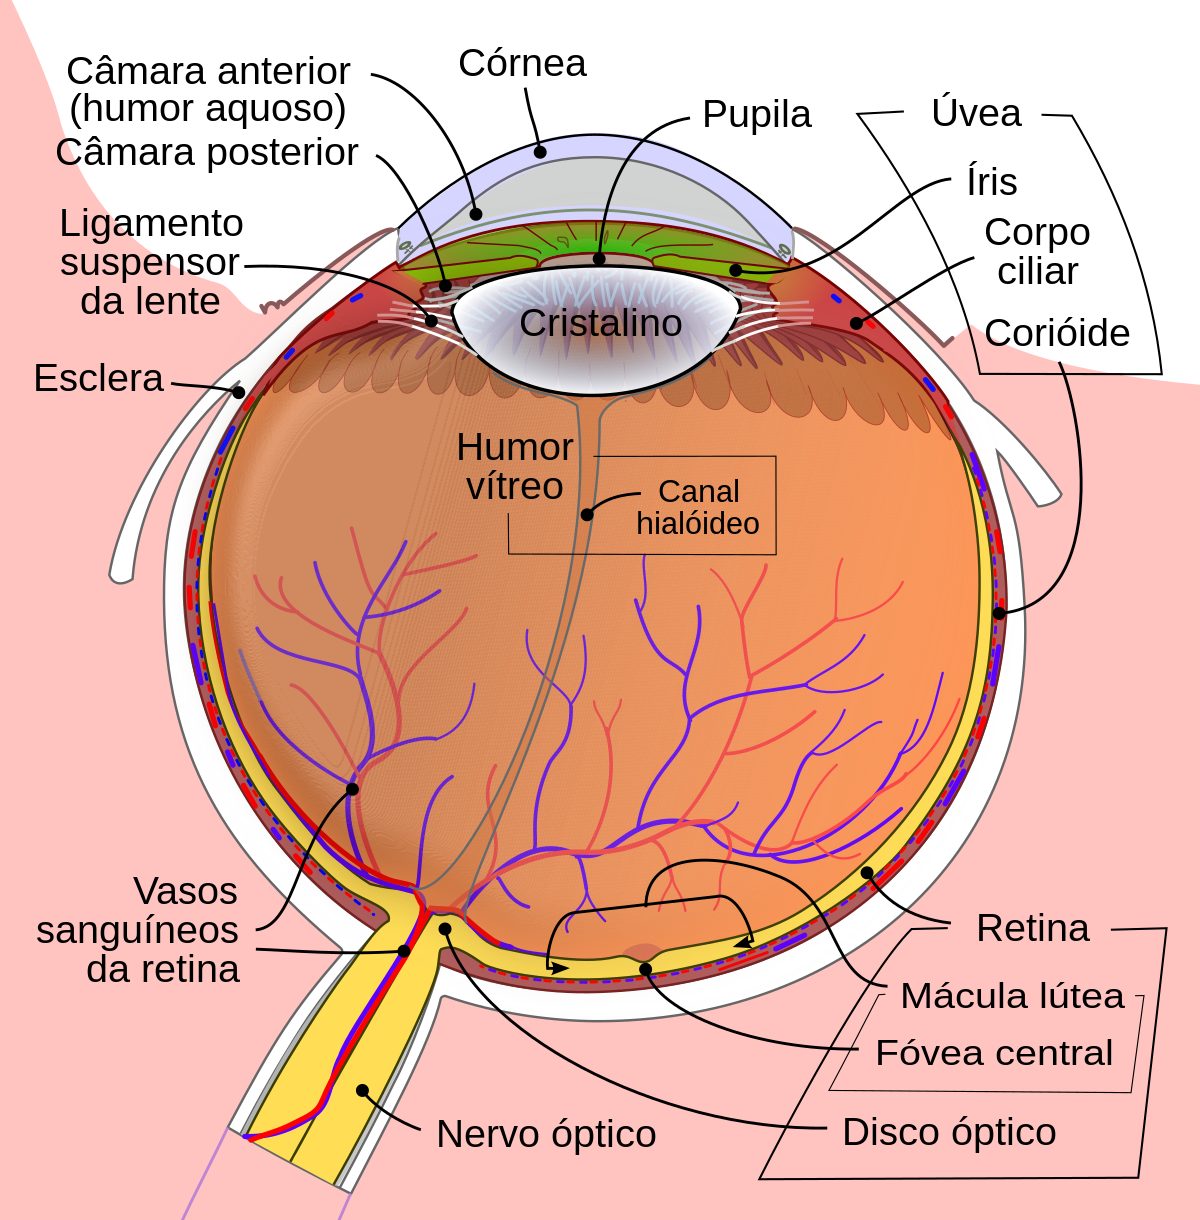
\includegraphics[width=0.8\textwidth]{images/5.png}
    \caption{Seção transversal do olho humano.}
    \label{fig:exemplo}
\end{figure}

\begin{itemize}
    \item A córnea é um tipo de tecido mais rígido, e é a parte que cobre a parte frontal do olho.
    \item Tem-se a esclera que encobre o restante do globo ocular.
    \item A coróide fica na parte de baixo da esclera e é responsável por fornecer oxigênio e nutrientes
    para o olho. A importância da coróide fica mais nítida ainda à medida que quaisquer danos
    a ela podem causar danos irreversíveis à visão.
    \item O coróide é dividido em duas partes: O corpo ciliar e o íris. O corpo ciliar é responsável
por produzir o humor aquoso, que é um líquido que preenche a câmara anterior do olho. O humor
    aquoso é responsável por manter a pressão do olho e nutrir a córnea e o cristalino. A íris é a
    parte colorida do olho, e é responsável por controlar a quantidade de luz que entra no olho.
    A pupíla de entrada pode variar de $2mm$ $f/8,3$ em ambientes bem iluminados até $8mm$ $f/2,1$ em
    ambientes escuros.
    \item O cristalino é composto de cerca de 65\% de água e 35\% de proteínas. Ele é responsável por
    focar a luz que entra no olho na retina. Em alguns casos extremos, o cristalino pode ser
    coberto por uma membrana chamada catarata, que pode causar cegueira. Ela é responsável por absrover
    cerca de 8\% do espectro da luz visível.
    \item A membrana mais interna, a retina é responsável por converter a luz que entra no olho em
    sinais elétricos que são enviados para o cérebro. A retina é composta de dois tipos de células
    fotorreceptoras: os cones e os bastonetes. Os cones são responsáveis por detectar a cor e
    funcionam melhor em ambientes bem iluminados. Os bastonetes são responsáveis por detectar a
    luz e funcionam melhor em ambientes escuros. Uma outra estrutura importante é a Fóvea, que é
    responsável por fornecer a visão central e é composta apenas por cones.
\end{itemize}
    Uma outra caracteristica importante do olho humano se diz respeito a cones e bastonetes, que são
    responsáveis por capturar a luz e transformar em sinais elétricos que são enviados para o cérebro.

    Cones: Em cada olho formam um total de cerca de 6 milhões de cones, e são responsáveis por capturar
    a luz e transformar em sinais elétricos que são enviados para o cérebro. Os cones são responsáveis
    por capturar a cor, e são responsáveis por capturar a luz em ambientes bem iluminados. Esse tipo
    de visão é chamada de visão fotópica.

    Bastonetes: Em cada olho formam um total de cerca de 120 milhões de bastonetes, e são responsáveis
    por capturar a luz e transformar em sinais elétricos que são enviados para o cérebro. Os bastonetes
    são responsáveis por capturar a luz em ambientes escuros, e são responsáveis por capturar a luz em
    ambientes escuros. Esse tipo de visão é chamada de visão escotópica.
\begin{figure}[H]
    \centering
    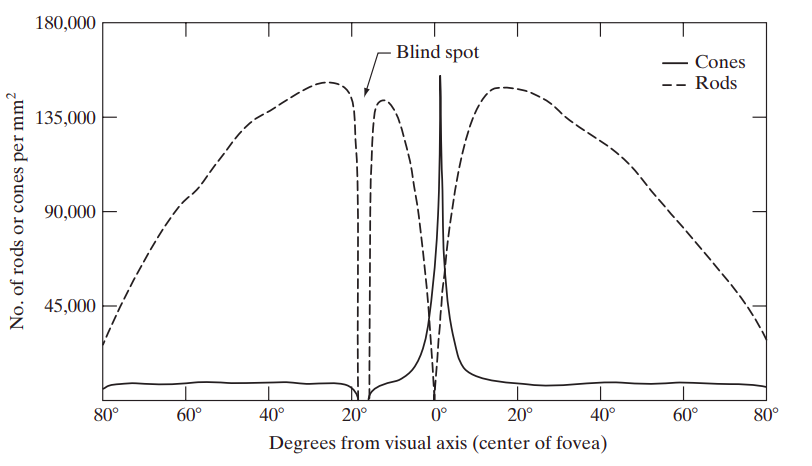
\includegraphics[width=0.8\textwidth]{images/6.png}
    \caption{Distribuição de cones e bastonetes na retina.}
    \label{fig:exemplo}
\end{figure}

A figura \ref{fig:exemplo} mostra a distribuição de cones e bastonetes na retina.

    \subsubsection{Formação da Imagem no Olho}

    Nas photografias as lentes possuem um ponto focal já estabelecido e também uma distância focal
    fixa, enquanto que em caso de filmes ou sensores digitais, a distância focal pode ser ajustada
    para focar em diferentes distâncias. Já no olho humano, a distância entre a lente e a região da
    imagem é fixa e o local de obtenção do foco é ajustado por meio de um músculo que altera a forma
    da lente.
    \begin{figure}[H]
        \centering
        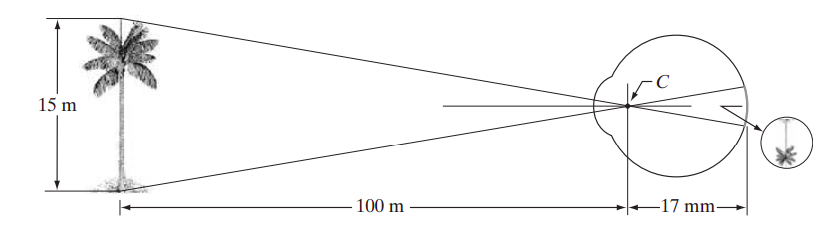
\includegraphics[width=0.8\textwidth]{images/7.png}
        \caption{Exemplo da formação da imagem no olho}
        \label{fig:exemplo}
    \end{figure}
    A distância entre o centro da lente e a retina é de aproximadamente 17mm, e a distância focal da
    lente é de aproximadamente 15mm. A imagem é formada na retina, e a imagem é invertida, e o cérebro
    é responsável por inverter a imagem.

    A figura \ref{fig:exemplo} mostra como obter dimensões das imagens formadas na retina. Por exemplo,
    suponha que uma pessoa está olhando uma árovre de 15 metros de altura a uma distância de 100metros.
    Chamando de $h$ a altura da imagem formada na retina a geometria obtida é a seguinte:
    \begin{equation}
        \frac{h}{17} = \frac{15}{100}
    \end{equation}
    Em outras palavras, a equação geral pode ser escrita como:
    \begin{equation}
        \frac{h}{d} = \frac{H}{D}
    \end{equation}
    Onde $h$ é a altura da imagem formada na retina, $d$ é a distância entre a lente e a retina, $H$ é
    a altura do objeto real, e $D$ é a distância entre o objeto e a lente.

    Como visto na seção anterior a imagem da retina é focada primariamente na fóvea, que é responsável
    por fornecer a visão central, e é composta apenas por cones.

    \subsubsection{Adaptação ao brilho e discriminação de cores}
    Devido as imagens digitais serem exibidas em tons discretos de valores, a habilidade de discriminar
    cores é uma tarefa a ser considerada para os olhos humanos. A distribuição de níveis de intensidade
    da luz que um sistema visual humano pode adaptar é vasta, a ordem chega a ser algo em torno de
    $10^{10}$ do limiar escotópico ao limite de ofuscamento. Existem algumas evidências de que a subjetividade
    do brilho é uma função logarítmica da intensidade da luz.
%reduza o tamanho da figura usando height
    \begin{figure}[h]
        \centering
        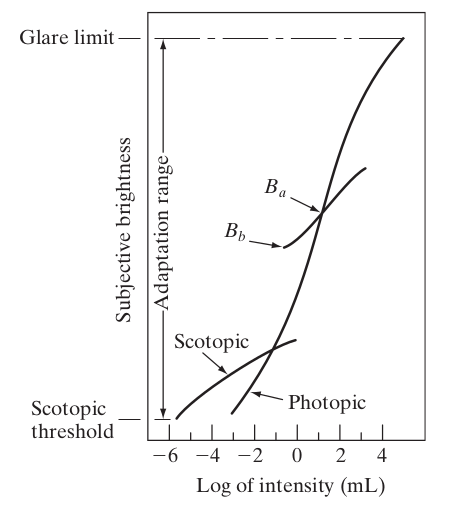
\includegraphics[width=10cm,height=10cm]{images/8.png}
        \caption{Curva de adaptação ao brilho}
        \label{fig:exemplo}
    \end{figure}
    A figura \ref{fig:exemplo} mostra a curva de adaptação ao brilho, que é uma curva logarítmica. A
    solida e longa curva representa a capacidade de adaptação do sistema. Uma visão fotópica é
    capaz de discriminar uma faixa de cerca de $10^{6}$. A transição escotópica-fotópica ocorre em
    torno de $0.001$ a $0.1$ Millilamberts.

    Para qualquer conjunto de condições de iluminação, o atual nível de sensibilidade a luz do sistema
    visual é chamado de adaptação ao brilho. Olhando para a figura \ref{fig:exemplo}, é possível ver
    que, por exemplo, o brilho $B_{a}$ representa uma curva de intersecção curta e representa
    a faixa de brilho subjetivo que o olho pode perceber quando está adaptado a este nível.
    Um fato sobre este intervalo é que ele é extremamente estreito, fechado, ter um nível $B_{B}$ no qual e abaixo do qual todos os estímulos são percebidos como indistintos
negros capazes. A parte superior da curva não é realmente restrita, mas, se for extendido ou
levado longe demais, perde seu significado porque intensidades muito mais altas simplesmente
elevar o nível de adaptação acima de $B_{a}$

    \begin{figure}[h]
        \centering
        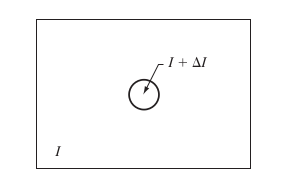
\includegraphics[width=10cm,height=10cm]{images/9.png}
        \caption{Experimento básico para caracterizar discriminação do brilho}
        \label{fig:Variação do I}
    \end{figure}

    Um outro fato interessante está relacionado com a proporção de Weber. Essa proporção vem da ideia
    da habilidade do olho humano em conseguir discriminar certas mudanças entre as alterações
    da intensidade da luz a um certo nível de adaptação considerada interessante.
    Considere um experimento usado para determinar a capacidade do sistema humano visual para discriminar
    o brilho. O experimento consiste em ter um olhar subjetivo a um plano uniformimente iluminado em uma área
    larga o suficiente para ocupar um campo de visão por inteiro. Essa área normalmente é difusa, como um vidro opaco, que
    é iluminada por uma fonte de luz com intensidade $I$, e pode ser variada. Nesse campo é adicionado um incremento a iluminação
    $\varDelta I$ em uma curta duração, ou seja um flash aparece em um circulo no centro uniforme iluminando o campo, conforme
    pode ser visualizado na figura \ref{fig:Variação do I}.
    Se o $\varDelta I$ não tiver brilho o suficiente o responsável pelo experimento irá dizer não, indicando uma mudança pouco
    perceptivel. A medida que $\varDelta I$ fica mais forte, o observador pode dar uma resposta positiva indicando uma mudança perspectiva na luminosidade. Até
    chegar no ponto de que a resposta é sempre sim. A quantidade de $\varDelta I_{c}/I$ onde $\varDelta I_{c}$ é o incremento da iluminação discriminavel em $50\%$ de todo o tempo
    de iluminação no fundo $I$ é o que chamamos de Proporção de Weber. Um pequeno valor de $\varDelta I_{c}/I$ indica uma grande porcentagem de mudança na intensidade requisitada.
    Isso representa uma discriminação pobre.
    \begin{figure}[H]
        \centering
        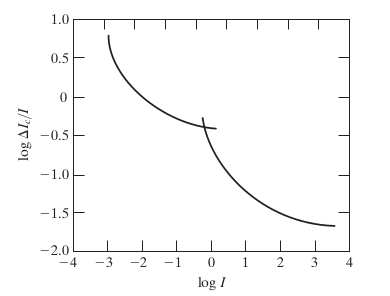
\includegraphics[width=10cm,height=10cm]{images/10.png}
        \caption{Curva de discriminação do brilho}
        \label{fig:Curv}
    \end{figure}

    Uma plotagem do log de $\varDelta I_{c}/I$ como uma função logaritmica de $I$ tem um formato que pode ser visualizado na
    figura \ref{fig:Curv}

    \begin{figure}[H]
        \centering
        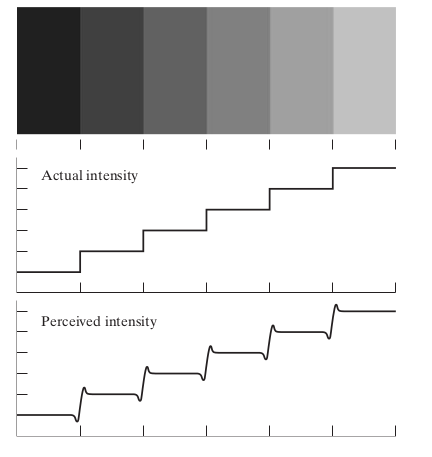
\includegraphics[width=8cm,height=8cm]{images/11.png}
        \caption{Ilustração do efeito Mach e ilustração da função de intensidade}
        \label{fig:mach}
    \end{figure}

    Efeito Mach: O efeito Mach é uma ilusão visual em que linhas paralelas parecem convergir em um ponto quando observadas
    em uma imagem bidimensional. No processamento digital de imagens, isso pode causar distorções perceptuais se não for considerado,
    exigindo técnicas específicas para corrigir ou mitigar o efeito, como correção de distorção ou uso de algoritmos de interpolação.

    Além disso o fenômeno abordado na figura \ref{fig:Curv} ilustra que o brilho recebido não é unicamente uma função de intensidade. Isso pode
    ser nitidamente visto na figura \ref{fig:mach}

    \begin{figure}[H]
        \centering
        
\includegraphics[width=10cm,height=10cm]{images/12.png}
        \caption{Exemplificação do efeito de contraste simultâneo}
        \label{fig:Contraste}
    \end{figure}

    Um outro fenômeno é o chamado de contraste simultaneo, isto esta associado ao fato de que uma região de cor cinza parece mais clara
    quando colocada em um fundo escuro, e mais escura quando colocada em um fundo claro. Isso é um fenômeno que ocorre devido a interação
    entre a região e o fundo. Esse fenômeno é ilustrado na figura \ref{fig:Contraste}

    \begin{figure}[H]
        \centering
        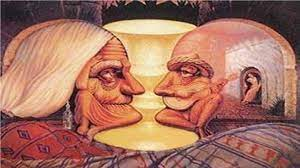
\includegraphics[width=10cm,height=10cm]{images/13.png}
        \caption{Exemplo de ilusões de óptica}
        \label{fig:ilusao}
    \end{figure}
    Outro exemplo até um tanto quanto divertido está associado aos fenômenos de ilusões de óptica.
    Essas ilusões são fenômenos que ocorrem quando o cérebro interpreta a informação visual de uma forma
    que não corresponde à realidade. Isso ocorre devido a uma série de fatores, como por exemplo, a
    forma como a luz incide sobre um objeto, a forma como a luz é refletida, entre outros.
    Alguns exemplos podem ser vistos na \ref{fig:ilusao}, onde pode ser visto no rosto do senhor
    um homem com uma especie de violão na mão, enquanto que no rosto da mulher pode ser visto uma mulher
    segurando uma especie de chapéu. Existem diversos tipos de ilusões de óptica.

    \subsection{Luz e o Espectro do campo Eletromagnetico}

    \begin{figure}[H]
        \centering
        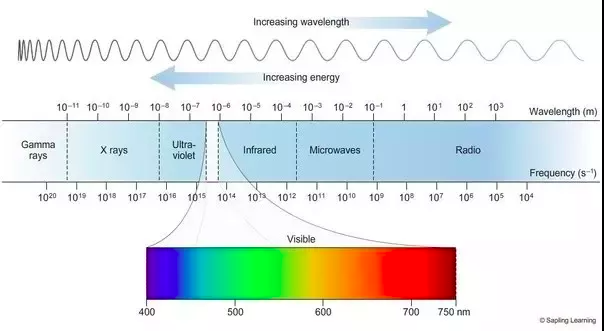
\includegraphics[width=15cm,height=15cm]{images/14.png}
        \caption{Espectro do campo eletromagnético}
        \label{fig:espectro}
    \end{figure}

    Conforme pode ser evidenciado na figura \ref{fig:espectro}, o espectro visível é apenas uma pequena
    parte do espectro eletromagnético. O campo do espectro eletromagnético pode ser representado por
    comprimentos de onda, frequencia ou energia. Comprimento de onda é representado por $\lambda$ e
    a frequência pode ser representada por $v$. A equação que relaciona comprimento de onda e frequência
    é dada por:
    \begin{equation}
        \lambda = \frac{c}{v}
    \end{equation}
    Onde $c$ é a velocidade da luz no vácuo, que é aproximadamente $3.0 \times 10^{8} m/s$. A energia
    de um fóton é dada por:
    \begin{equation}
        E = hv
        \label{eq:energia}
    \end{equation}
    Onde $h$ é a constante de Planck, que é aproximadamente $6.626 \times 10^{-34} J.s$. A energia de
    um fóton é diretamente proporcional a frequência, e inversamente proporcional ao comprimento de onda.

    A frequência é abordada em Hertz(Hz), e é uma medida de ciclos por segundo. A frequência é uma
    medida de quão rápido um fóton oscila.

    Ondas eletromagnéticas podem ser vistas como propagação sinusoidal de campos elétricos e magnéticos
que são perpendiculares entre si e perpendiculares a direção de propagação da onda.

    \begin{figure}[h]
    \begin{adjustwidth}{-5cm}{}
        \centering
        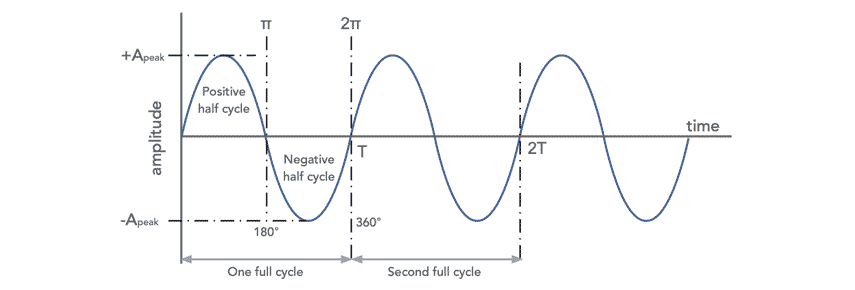
\includegraphics[]{images/15.png}
        \caption{Exemplo de onda sinusoidal}
        \label{fig:onda}
    \end{adjustwidth}
\end{figure}

    Cada pacote de energia é chamado de fóton. É visto na equação \ref{eq:energia} que a energia de um
    fóton é diretamente proporcional a frequência, e inversamente proporcional ao comprimento de onda.

    Com essas informações em mente tem-se um fato: Por que ondas de raio gamma são mais perigosas que
    ondas de rádio? A resposta está na equação \ref{eq:energia}, que mostra que a energia de um fóton
    é diretamente proporcional a frequência, e inversamente proporcional ao comprimento de onda. Com
    isso, ondas de raio gamma possuem mais energia que ondas de rádio, e com isso são mais perigosas.

    A faixa de cores pode ser vista na imagem \ref{fig:espectro}, e é uma faixa que vai de aproximadamente
    $400nm$ até $700nm$. A luz branca é composta por todas as cores, e a cor branca é a cor que é
    percebida quando todas as cores são misturadas. As cores que são enxergadas são as cores que são
    refletidas pelos objetos.

    \subsection{Detecção e Aquisição de imagem}

    A grande maioria das imagens analisadas são generadas pela combinação de luz e sensores. A luz
    atua como um sinal que é capturado por um sensor, e é convertido em um sinal elétrico que é
    processado por um computador. Por exemplo um exame de raio-x é um exemplo de imagem que é gerada
    pela combinação de luz e sensores.

    \begin{figure}[H]
        \centering
        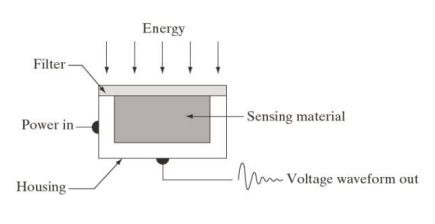
\includegraphics[]{images/16.png}
        \caption{Exemplo de um sensor de imagem simples}
        \label{fig:sensor}
    \end{figure}

    Observando a imagem \ref{fig:sensor}, vê-se que a energia luminosa é passada por uma espécie de filtro que
    é responsável por separar a luz em suas componentes de cor, e cada componente de cor é passada
    por um sensor que é responsável por converter a luz em um sinal elétrico.

    Existem alguns outros sensores, como por exemplo, Sensores Lineares e Sensores de Matriz.

\end{document}
